\section{Intraprocedural Profiling}

{\em Path profiling} is a powerful {\em intraprocedural} methodology for identifying performance bottlenecks in a program, and has received considerable attention in the last 15 years for its practical relevance. The well-known Ball and Larus numbering algorithm~\cite{Ball96} can efficiently encode {\em acyclic} paths that are taken across the control-flow graph of a function. Previous attempts to extend it to {\em cyclic} paths - thus spanning multiple loop iterations - to capture more optimization opportunities, are based on rather complex algorithms that incur severe performance overheads even for short cyclic paths. In this thesis we present a new, data-structure based approach to {\em multi-iteration} path profiling built on top of the original Ball-Larus numbering technique. Starting from the observation that a cyclic path can be described as a concatenation of Ball-Larus acyclic paths, we show how to accurately profile all executed paths obtained as a concatenation of up to $k$ Ball-Larus paths, where $k$ is a user-defined parameter.

%{\em Path profiling} is a powerful {\em intraprocedural} methodology for identifying performance bottlenecks in a program, and has received considerable attention in the last 15 years for its practical relevance. The well-known Ball and Larus algorithm~\cite{Ball96} for {\em intraprocedural} path profiling can efficiently encode {\em acyclic} paths that are taken across the control-flow graph of a function. Previous attempts to extend it to encode {\em cyclic} paths, and thus to span multiple loop iterations in order to capture more optimization opportunities, are based on rather complex algorithms that incur severe performance overheads even for short cyclic paths. In this thesis we present a new, data-structure based approach to {\em multi-iteration} path profiling built on top of the original Ball-Larus numbering technique. Starting from the observation that any cyclic path can be described as a concatenation of Ball-Larus acyclic paths, we show how to accurately profile all executed paths obtained as a concatenation of up to $k$ Ball-Larus paths, where $k$ is a user-defined parameter.

%We provide examples showing that this method can reveal optimization opportunities that acyclic-path profiling would miss, and we present an extensive experimental investigation on a large variety of Java benchmarks in the Jikes RVM. Experiments show that our approach can be even faster than a hash table-based implementation of the Ball-Larus algorithm due to fewer operations on smaller tables, producing compact representations of cyclic paths even for large values of $k$.

\subsection{Motivation and Contributions}

Path profiling associates performance metrics, usually frequency counters, to paths taken in the control flow graph of a routine. Identifying the hottest paths can direct optimizations to portions of the code where most resources are consumed, often yielding significant speedups. For instance, trace scheduling can be used to increase instruction-level parallelism along frequently executed paths~\cite{Fisher81,Young98}. Basic-block and edge profiles, albeit inexpensive and widely available, may not correctly predict frequencies of overlapping paths, and are thus inadequate for such optimizations. 

The seminal paper by Ball and Larus~\cite{Ball96} introduced a simple and elegant path profiling technique. The main idea was to implicitly number all possible acyclic paths in the control flow graph so that each path is associated with a unique compact path identifier (ID). The authors showed that path IDs can be efficiently generated at run time and can be used to update a table\footnote{Large routines can have too many potential paths to use an array of counters. In this case, a slower (but more space-efficient) hash table is used to record only paths that actually execute~\cite{Ball96}.} of frequency counters. Although in general the number of acyclic paths may grow exponentially with the graph size, in typical control flow graphs this number is usually small enough to fit in current machine word-sizes, making this approach very effective in practice.

While the original Ball-Larus approach was restricted to acyclic paths obtained by cutting paths at loop back edges, profiling paths that span consecutive loop iterations is a desirable, yet difficult, task that can yield better optimization opportunities. Consider, for instance, the problem of eliminating redundant executions of instructions, such as loads and stores~\cite{Bodik99}, conditional jumps~\cite{Bodik97}, expressions~\cite{Bodik98,Bodik04}, and array bounds checks~\cite{Bodik00}. A typical situation is that the same instruction is redundantly executed at each loop iteration, which is particularly common for arithmetic expressions and load operations~\cite{Bodik04,Bodik99}. To identify such redundancies, paths that extend across loop back edges need to be profiled. Another application is trace scheduling~\cite{Young98}: if a frequently executed cyclic path is found, compilers may unroll the loop and perform trace scheduling on the unrolled portion of code. The benefits of multi-iteration path profiling are discussed in depth in~\cite{Tallam04}.

Different authors have proposed techniques to profile cyclic paths by modifying the original Ball-Larus path numbering scheme in order to identify paths that extend across multiple loop iterations~\cite{Tallam04,Roy09,Li12}. Unfortunately, all known solutions require rather complex algorithms that incur severe performance overheads even for short cyclic paths, leaving the interesting open question of finding simpler and more efficient alternative methods.

\paragraph*{Contributions.} In this thesis, we present a novel, data structure-based approach to multi-iteration path profiling. Our method stems from the observation that any cyclic path in the control flow graph of a routine can be described as a concatenation of Ball-Larus acyclic paths (BL paths). In particular, we show how to accurately profile {\em all executed paths} obtained as a concatenation of up to $k$ BL paths, where $k$ is a user-defined parameter. We reduce multi-iteration path profiling to the problem of counting $n$-grams, i.e., contiguous sequences of $n$ items from a given sequence. To compactly represent collected profiles, we organize them in a forest of prefix trees (or tries)~\cite{Fredkin60} of depth up to $k$, where each node is labeled with a BL path, and paths in a tree represent concatenations of BL paths that were actually executed by the program, along with their frequencies. We also present an efficient construction algorithm based on a variant of the \ksf\ data structure presented in~\cite{Ausiello12}. 

\subsection{Approach}

Differently from previous techniques~\cite{Tallam04,Roy09,Li12}, which rely on modifying the Ball-Larus path numbering to cope with cycles, our method does not	require any modification of the original numbering technique described in~\cite{Ball96}.

\ifdefined\noauthorea
\begin{wrapfigure}[19]{l}{0.5\textwidth}
\vspace{-3mm}
\centering
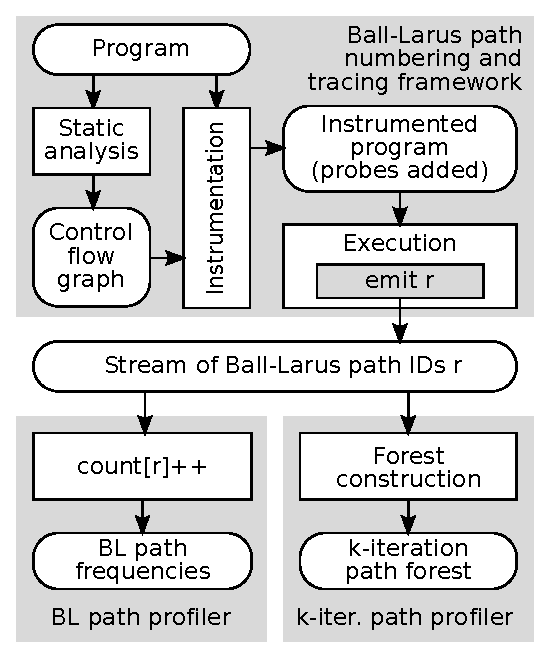
\includegraphics[width=0.433\textwidth]{figures/kblpp-approach/kblpp-approach.eps}
\captionsetup{width=.47\textwidth}
\caption{\protect\label{fig:kblpp-approach} Overview of our approach: Ball-Larus profiling versus k-iteration path profiling, cast in a common framework.
%Overview of our approach: classical Ball-Larus profiling versus k-iteration path profiling, cast in a common framework.
}
%\vspace{2mm}
\end{wrapfigure}
\noindent
\fi

\vspace{-2mm}
\noindent The main idea behind our approach is to fully decouple the task of tracing Ball-Larus acyclic paths at run time from the task of concatenating and storing them in a data structure to keep track of multiple iterations.

\myfigure\ref{fig:kblpp-approach} illustrates from a high-level point of view our two-stage process:
\begin{enumerate}[parsep=0pt,itemsep=3pt,topsep=5pt]
\item instrumentation and execution of the program to be profiled (top);
\item profiling of paths (bottom).
\end{enumerate}
We let the Ball-Larus profiling algorithm issue a stream of BL path IDs, where each ID is generated when a back edge in the control flow graph is traversed or the current procedure is abandoned. As a consequence of this modular approach, our method can be implemented on top of existing Ball-Larus path profilers, making it simpler to code and maintain.

%\vspace{1em}

%\noindent
The first phase is almost identical to the original approach described in~\cite{Ball96}. The target program is statically analyzed and a control flow graph (CFG) is constructed for each routine of interest. The CFG is used to instrument the original program by inserting probes, which allow paths to be traced at run time. When the program is executed, taken acyclic paths are identified using the inserted probes. The main difference with the Ball-Larus approach is that, instead of directly updating a frequency counters table here, we emit a stream of path IDs, which is passed along to the next stage of the process. This allows us to decouple the task of tracing taken paths from the task of profiling them. 

The profiling phase can be either the original hash table-based method of~\cite{Ball96} used to maintain BL path frequencies
%for larger programs
(bottom-left of \myfigure\ref{fig:kblpp-approach}), or other approaches such as the one we propose, i.e., profiling concatenations of BL paths in a forest-based data structure (bottom-right of \myfigure\ref{fig:kblpp-approach}). Different profiling methods can be therefore cast into a common framework, increasing flexibility and helping us make more accurate comparisons.

We start the description of our approach with a brief overview of the Ball-Larus path tracing technique, which we use as the first stage of our profiling technique.

\subsubsection*{Ball-Larus Path Tracing Algorithm}

The Ball-Larus path profiling (BLPP) technique~\cite{Ball96} identifies each acyclic path that is executed in a routine. Paths start on the method entry and terminate on the method exit. Since loops make the CFG cyclic, loop back edges are substituted by a pair of dummy edges: the first one from the method entry to the target of the loop back edge, and the second one from the source of the loop back edge to the method exit. After this transformation, which preserves the number of acyclic paths and is reversible, the CFG of a method becomes a directed acyclic graph (DAG), thus acyclic paths can be easily enumerated.

\ifdefined\noauthorea
\begin{figure}[h!]
\IncMargin{2em}
\begin{algorithm}[H]
\DontPrintSemicolon
\LinesNumbered
\SetAlgoNoLine
\SetNlSkip{1em} 
\Indm\Indmm
\hrulefill\\
$\mathbf{procedure} \> \> \texttt{bl\_path\_numbering}$():\;
\vspace{1mm}
\everypar={\nl}
\Indp\Indpp
\ForEach{$\textsf{\rm basic block}$ $v$ $\textsf{\rm in reverse topological order}$}{
    \eIf{$v$ $\textsf{\rm is the exit block}$}{
	numPaths($v$) $\gets 1$\;
    }{
	numPaths($v$) $\gets 0$\;
	\ForEach{$\textsf{\rm outgoing edge}$ $e = (v, w)$}{
	    val($e$) = numPaths($v$) \;
	    numPaths($v$) += numPaths($w$) \;
	}
    }
}
\vspace{-2mm}
\Indm\Indmm
\nonl\hrulefill\vspace{1mm}\\
\DecMargin{5em}
\caption{\label{alg:kblpp-bl-numbering} The Ball-Larus path numbering algorithm.}
\IncMargin{3em}
\end{algorithm}
\end{figure}

\else
\begin{figure}[h!]
\caption{\label{alg:kblpp-bl-numbering} The Ball-Larus path numbering algorithm.}
\begin{small}
\begin{minipage}{0.9\textwidth}
\hrulefill\\
\textbf{procedure} {\tt bl\_path\_numbering}(): \\
\vspace{-2mm}

1. ~~ \textbf{foreach} basic block $v$ in reverse topological order \textbf{do}\\
2. ~~ ~~~~ \textbf{if} $v$ is the exit block \textbf{then}\\
3. ~~ ~~~~ ~~~~ numPaths($v$) $\gets 1$\\
4. ~~ ~~~~ \textbf{else}\\
5. ~~ ~~~~ ~~~~ numPaths($v$) $\gets 0$\\
6. ~~ ~~~~ ~~~~ \textbf{foreach} outgoing edge $e = (v, w)$ \textbf{do}\\
7. ~~ ~~~~ ~~~~ ~~~~ val($e$) = numPaths($v$)\\
8. ~~ ~~~~ ~~~~ ~~~~ numPaths($v$) += numPaths($w$)\\
9. ~~ ~~~~ ~~~~ \textbf{end}\\
10. ~~ ~~~~ \textbf{end}\\
11. ~~ \textbf{end}\\
\vspace{-1mm}
\hrulefill
\vspace{-2mm}
\end{minipage}
\end{small}
\end{figure}

\fi

\ifdefined\noauthorea
\begin{figure}[ht]
\begin{center}
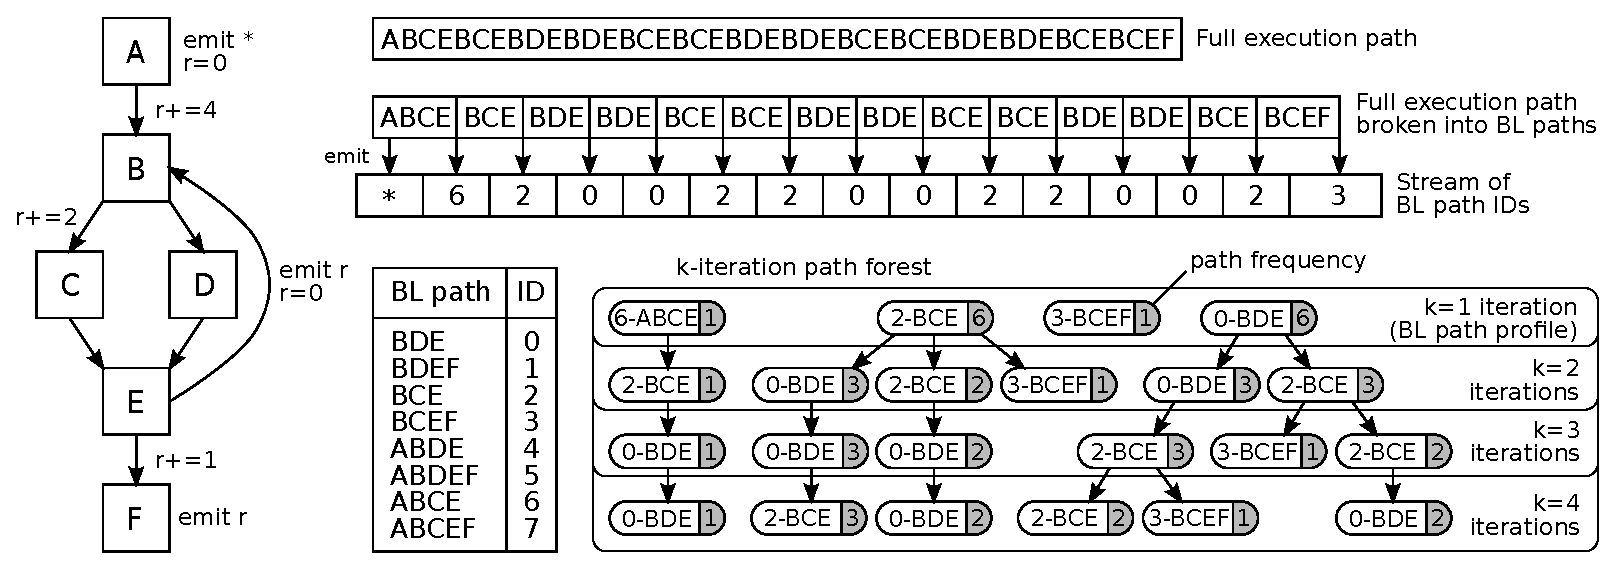
\includegraphics[width=\textwidth]{figures/kblpp-example/kblpp-example.eps}
\caption{\protect\label{fig:kblpp-example} Control flow graph (CFG) with Ball-Larus instrumentation modified to emit acyclic path IDs to an output stream and running example of our approach that shows a 4-iteration path forest (4-IPF) for a possible small execution trace. Loop back edges in the CFG have been restored after the path numbering phase.
}
\end{center}
\end{figure}
\fi

\ifauthorea{\newline}{}
\noindent The Ball-Larus path numbering algorithm
\ifauthorea{, shown in \myalgorithm\ref{alg:kblpp-bl-numbering},}{(\myalgorithm\ref{alg:kblpp-bl-numbering})}
assigns a value $val(e)$ to each edge $e$ of the CFG such that, given N acyclic paths, the sum of the edge values along any entry-to-exit path is a unique numeric ID in [0, N-1]. A CFG example (untransformed) and the corresponding path IDs are shown in \myfigure\ref{fig:kblpp-example}: notice that there are eight distinct acyclic paths, numbered from 0 to 7, starting either at the method's entry $A$, or at loop header $B$ (target of back edge $(E,B)$).

BLPP places instrumentation on edges to compute a unique path number for each possible path that is taken at run time. In particular, it maintains a variable {\tt r}, called {\em probe} or {\em path register}, to compute the path number. Variable {\tt r} is first initialized to zero upon method entry and is then updated as edges are traversed. When an edge that reaches the method exit is executed, or a back edge is traversed, variable {\tt r} represents the unique ID of the taken path. As observed, instead of using the path ID {\tt r} to increase the associated path frequency counter ({\tt count[r]++}), we defer the profiling stage by emitting the path ID to an output stream ({\tt emit r}). To support profiling over multiple invocations of the same routine, we annotate the stream with the special marker $*$ to denote a routine entry event. Instrumentation code for our CFG example is shown on the left of \myfigure\ref{fig:kblpp-example}.

\subsubsection*{$k$-iteration Path Profiling}
The second stage of our profiling technique takes as input the stream of BL path IDs generated by the first stage and uses it to build a data structure that keeps track of the frequencies of {\em each and every distinct taken path} consisting of the concatenation of up to $k$ BL paths, where $k$ is a user-defined parameter. This problem is equivalent to counting all $n$-grams, i.e., contiguous sequences of $n$ items from a given sequence of items, for each $n\le k$. Our solution is based on the notion of {\em prefix forest}, which compactly encodes a list of sequences by representing repetitions and common prefixes only once. A prefix forest can be defined as follows:

\begin{definition}[Prefix forest]
\label{de:kblpp-prefix-forest}
Let $L=\langle x_1, x_2, \ldots, x_q\rangle$ be any list of finite-length sequences over an alphabet $H$. The {\em prefix forest} ${\cal F}(L)$ of $L$ is the smallest labeled forest such that, $\forall$ sequence $x=\langle a_1, a_2, \ldots, a_n\rangle$ in $L$ there is a path $\pi=\langle \nu_1, \nu_2, \ldots, \nu_n\rangle$ in ${\cal F}(L)$ where $\nu_1$ is a root and $\forall j\in[1,n]${\em :}
\begin{enumerate}
\item $\nu_j$ is labeled with $a_j$, i.e., $\ell(\nu_j)=a_j\in H$;
\item $\nu_j$ has an associated counter $c(\nu_j)$ that counts the number of times sequence $\langle a_1, a_2, \ldots, a_j\rangle$ occurs in $L$.
\end{enumerate}
\end{definition}

\noindent By \mydefinition\ref{de:kblpp-prefix-forest}, each sequence in $L$ is represented as a path in the forest, and node labels in the path are exactly the symbols of the sequence, in the same order. The notion of minimality implies that, by removing even one single node, there would be at least one sequence of $L$ not counted in the forest. Observe that there is a distinct root in the forest for each distinct symbol that occurs as first symbol of a sequence.

%\paragraph*{k-iteration path forest.}
The output of the second stage of our profiling technique is a prefix forest, which we call {\em k-Iteration Path Forest} (\kipf), that compactly represents all observed contiguous sequences of up to $k$ BL path IDs:

\begin{definition}[$k$-Iteration Path Forest]
\label{de:kipf}
Given an input stream $\Sigma$ representing a sequence of BL path IDs and $*$ markers, the {\em k-Iteration Path Forest} (\kipf) of $\Sigma$ is defined as $\kipf={\cal F}(L)$, where $L=\{$\,list of all $n$-grams of $\Sigma$ that do not contain $*$, with $n\le k\,\}$.
\end{definition}

\noindent By \mydefinition\ref{de:kipf}, the \kipf\ is the prefix forest of all consecutive subsequences of up to $k$ BL path IDs in $\Sigma$. Each path $\langle\nu_1, \nu_2, ..., \nu_q\rangle$ in the forest, with $q\le k$, corresponds thus to a consecutive sequence of items $\langle\ell(\nu_1), \ell(\nu_2), ..., \ell(\nu_q)\rangle$ that occurs in $\Sigma$.

\begin{example} \myfigure\ref{fig:kblpp-example} provides an example showing the 4-IPF constructed for a small sample execution trace consisting of a sequence of 44 basic blocks encountered during one invocation of the routine described by the control flow graph on the left. Notice that the full (cyclic) execution path starts at the entry basic block $A$ and terminates on the exit basic block $F$. The first stage of our profiler issues a stream $\Sigma$ of BL path IDs that are obtained by emitting the value of the probe register $r$ each time a back edge is traversed, or the exit basic block is executed. Observe that the sequence of emitted path IDs induces a partition of the execution path into Ball-Larus acyclic paths. Hence, the sequence of executed basic blocks can be fully reconstructed from the sequence $\Sigma$ of path IDs.

The 4-IPF built in the second stage contains exactly one tree for each of the 4 distinct BL path IDs (0, 2, 3, 6) that occur in the stream. We observe that path frequencies in the first level of the 4-IPF are exactly those that traditional Ball-Larus profiling would collect. The second level contains the frequencies of taken paths obtained by concatenating 2 BL paths, etc. Notice that the path labeled with $\langle 2, 0, 0, 2\rangle$ in the 4-IPF, which corresponds to the path $\langle B, C, E, B, D, E, B, D, E, B, C, E \rangle$ in the control flow graph, is a 4-gram that occurs 3 times in $\Sigma$ and is one of the most frequent paths among those that span from 2 up to 4 loop iterations.
\end{example}

\paragraph*{Properties.} 
A \kipf\ has some relevant properties:
\begin{enumerate}
\item $\forall$ nodes $\alpha\in$ $k$-IPF, $k>0$: $$c(\alpha)\ge\sum_{\beta_i\,:\,edge\,(\alpha,\beta_i)\in\,k\mbox{\scriptsize-IPF}} c(\beta_i);$$
\item $\forall k>0$, $k$-IPF $\subseteq$ ($k+1$)-IPF.
\end{enumerate}

\noindent By Property~1, since path counters are non-negative, they are monotonically non-increasing as we walk down the tree. The inequality $\ge$ in Property~1 may be strict ($>$) if the execution trace of a routine invocation does not end at the exit basic block; this may be the case when a subroutine call is performed at an internal node of the CFG. 

Property~2 implies that, for each tree $T_1$ in the $k$-IPF there is a tree $T_2$ in the $(k+1)$-IPF such that $T_2$ is equal to $T_1$ after removing leaves at level $k+1$.
%, i.e., $T_1$ is a subtree of $T_2$ starting at the root of $T_2$.
Notice that a 1-IPF includes only acyclic paths and yields exactly the same counters as a Ball-Larus profiler~\cite{Ball96}.

%~\cite{}

\subsection{Algorithms}

We observe that building explicitly a \kipf\ concurrently with a program's execution would require updating up to $k$ nodes for each traced BL path: indeed, this may considerably slow down the program even for small values of $k$. Given a stream of BL path IDs, we show that a \kipf\ profile can be constructed by maintaining an intermediate data structure that can be updated quickly, and then converting it into a \kipf\
%more efficiently
when the stream is over. As intermediate data structure, we use a variant of the {\em $k$-slab forest} (\ksf) introduced in~\cite{Ausiello12}.

\paragraph*{Main idea.} The variant of the \ksf\ we present in this paper is tailored to keep track of all the $n$-grams from a sequence of symbols, for all $n\le k$. The organization of our data structure stems from the following simple observation: if we partition a sequence into chunks of length $k-1$, then any subsequence of length up to $k$ will be entirely contained within two consecutive chunks of the partition. The main idea is therefore to consider all subsequences that start at the beginning of a chunk and terminate at the end of the next chunk, and join them in a prefix forest. Such a forest will contain information for all subsequences of length up to $k$ starting in an arbitrary position of the stream, and also for subsequences of length up to $2k-2$ starting at the beginning of a chunk. Moreover, this forest will contain a distinct tree for each distinct symbol that appears at the beginning of any chunk.

The partition of the sequence into chunks induces a division of the forest into upper and lower regions ({\em slabs}) of height up to $k-1$. As we will see later on in this section, this organization implies that the \ksf\ can be constructed on-line as stream items are revealed to the profiler by adding or updating up to two nodes of the forest at a time, instead of $k$ nodes as we would do if we incremented explicitly the frequencies of $n$-grams as soon as they are encountered in the stream.

%The following example applies the concepts described above to a stream of BL path IDs.

\ifdefined\noauthorea
\begin{figure}[ht]
\begin{center}
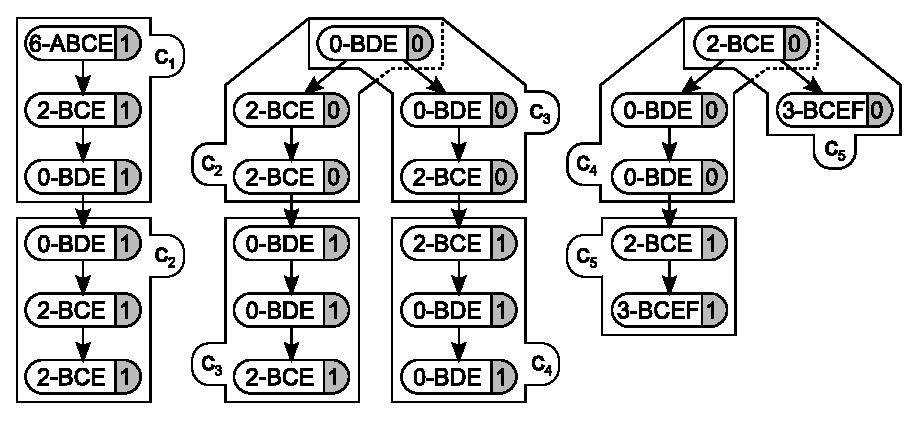
\includegraphics[width=0.8\textwidth]{figures/kblpp-ksf/kblpp-ksf.eps}
\caption{\protect\label{fig:kblpp-ksf} 4-SF resulting from the execution trace of Figure~\ref{fig:kblpp-example}.}
\vspace{-2mm}
\end{center}
\end{figure}
\fi

\begin{example} 
\label{ex:kblpp-ksf}
Let us consider again the example given in \myfigure\ref{fig:kblpp-example}. For $k=4$, we can partition the stream into maximal chunks of up to $k-1=3$ consecutive BL path IDs as follows: $$\Sigma=\langle *, \underbrace{\framebox{6, 2, 0}}_{c_1}, \underbrace{\framebox{0, 2, 2}}_{c_2}, \underbrace{\framebox{0, 0, 2}}_{c_3}, \underbrace{\framebox{2, 0, 0}}_{c_4}, \underbrace{\framebox{2, 3}}_{c_5}\rangle.$$
The $4$-SF of $\Sigma$, defined in terms of chunks $c_1, \ldots, c_5$, is shown in \myfigure\ref{fig:kblpp-ksf}. Notice for instance that 2-gram $\langle 0,0\rangle$ occurs three times in $\Sigma$ and five times in the $4$-SF. However, only three of them end in the bottom slab and hence are counted in the frequency counters.
\end{example}

\noindent To obtain a \kipf\ starting from the \ksf, for each BL path ID that appears in the stream we
%will
eventually construct the set of nodes in the \ksf\ associated with it and join the subsequences of length up to $k$ starting from those nodes into a prefix forest.

%Before presenting our algorithms, we provide a formal definition of the \ksf:

\begin{definition}[$k$-slab forest]
\label{def:kblpp-ksf}
Let $k\ge 2$ and let $c_1, c_2, c_3, \ldots,$ $c_m$ be the chunks of $\Sigma$ obtained by: (1) splitting $\Sigma$ at $*$ markers, (2) removing the markers, and (3) cutting the remaining subsequences every $k-1$ consecutive items. The {\em $k$-slab forest} (\ksf) of $\Sigma$ is defined as $\ksf={\cal F}(L)$, where $L=\{$list of all prefixes of $c_1\cdot c_2$ and all prefixes of length $\ge k$ of $c_i\cdot c_{i+1}$, $\forall i\in [2,m-1]\}$ and $c_i\cdot c_{i+1}$ denotes the concatenation of $c_i$ and $c_{i+1}$.
\end{definition}

\noindent By \mydefinition\ref{def:kblpp-ksf}, since each chunk $c_i$ has length up to $k-1$, then a \ksf\ has at most $2k-2$ levels and depth $2k-3$. As observed above, the correctness of the \ksf\ representation stems from the fact that, since each occurrence of an $n$-gram with $n\le k$ appears in $c_i\cdot c_{i+1}$ for some $i$, then there is a tree in the \ksf\ representing it.

\begin{example} In accordance with \mydefinition\ref{def:kblpp-ksf}, the forest of \myfigure\ref{fig:kblpp-ksf} for the stream of \myexample\ref{ex:kblpp-ksf} is ${\cal F}(L)$, where $L=\langle$ $
\langle 6\rangle, 
\langle 6, 2\rangle, 
\langle 6, 2, 0\rangle, 
\langle 6, 2, 0, 0\rangle, 
\langle 6, 2, 0, 0,$
$
2\rangle,
\langle 6, 2, 0, 0, 2, 2\rangle,
%\langle 0\rangle, 
%\langle 0, 2\rangle, 
%\langle 0, 2, 2\rangle, 
\langle 0, 2, 2, 0\rangle, 
\langle 0, 2, 2, 0, 0\rangle, 
\langle 0, 2, 2, 0, 0, 2\rangle,
%\langle 0\rangle,
%\langle 0, 0\rangle,
%\langle 0, 0, 2\rangle,
\langle 0, 0, 2, 2\rangle,
\langle 0, 0,2,$ $2, 0\rangle,
\langle 0,$
$
0, 2, 2, 0, 0\rangle,
%\langle 2\rangle,
%\langle 2, 0\rangle,
%\langle 2, 0, 0\rangle,
\langle 2, 0, 0, 2\rangle,
\langle 2, 0, 0, 2, 3\rangle
%\langle 2\rangle,
%\langle 2, 3\rangle
\rangle$.
\end{example}

\paragraph*{k-SF construction algorithm.} Given a stream $\Sigma$ formed by BL path IDs and $*$ markers, which we remind the reader denote routine entry events, the \ksf\ of $\Sigma$ can be constructed by calling the procedure {\tt process\_bl\_path\_id}$(r)$ shown in \myalgorithm\ref{alg:kblpp-ksf-algorithm} on each item $r$ of $\Sigma$. The streaming algorithm, which is a variant of the \ksf\ construction algoritm given in~\cite{Ausiello12} for the different setting of bounded-length calling contexts, keeps the following information:

\ifdefined\noauthorea
%\ifx\noauthorea\undefined
\begin{figure}[ht!]
\IncMargin{2em}
\begin{algorithm}[H]
\DontPrintSemicolon
\LinesNumbered
\SetAlgoNoLine
\SetNlSkip{1em} 
\Indm\Indmm
\hrulefill\\
$\mathbf{procedure} \> \> \texttt{process\_bl\_path\_id}$($r$):\;
\vspace{1mm}
\everypar={\nl}
\Indp\Indpp
\If{$r=*$}{
  $n\gets 0$\;
  $\tau\gets{\tt null}$\;
  \Return{}
}
%\eIf{$n$ $\bf{\textsf{\tt mod}}$ $(k-1)=0$}{
\eIf{$n$ $\textsf{\rm mod}$ $(k-1)=0$}{
  $\beta\leftarrow \tau$\;
  $\tau\,\leftarrow\,${\tt find$(R,r)$}\;
  \If{$\tau = \textsf{\tt null}$}{
    add root $\tau$ with $\ell(\tau)=r$ and $c(\tau)=0$ to \ksf\ and $R$\;
  }
}{
  find child $\omega$ of node $\tau$ with label $\ell(\omega)=r$\;
  \If{$\omega$ = \textsf{\tt null}}{
    add node $\omega$ with $\ell(\omega)=r$ and $c(\omega)=0$ to \ksf\;
    add arc $(\tau,\omega)$ to \ksf\;
  }
  $\tau\leftarrow \omega$\;
}
\eIf{$\beta\neq{\textsf{\tt null}}$}{
  find child $\upsilon$ of node $\beta$ with label $\ell(\upsilon)=r$\;
  \If{$\upsilon = \textsf{\tt null}$}{
    add node $\upsilon$ with $\ell(\upsilon)=r$ and $c(\upsilon)=0$ to \ksf\;
    add arc $(\beta,\upsilon)$ to \ksf\;
  }
  $\beta\leftarrow \upsilon$\;
  $c(\beta)\gets c(\beta)+1$\;
}{
  $c(\tau)\gets c(\tau)+1$\;
}
$n\gets n+1$\;
\vspace{-2mm}
\Indm\Indmm
\nonl\hrulefill\vspace{1mm}\\
\DecMargin{1.5em}
\caption{\label{alg:kblpp-ksf-algorithm} Stream processing algorithm for \ksf\ construction.}
%\IncMargin{0em}
\DecMargin{0.5em}
\end{algorithm}
\end{figure}

\else
\begin{figure}[ht]
\caption{\label{alg:kblpp-ksf-algorithm} Stream processing algorithm for \ksf\ construction.}
\begin{small}
\begin{minipage}{0.9\textwidth}
\hrulefill\\
\algmissing\

\vspace{-1mm}
\hrulefill
\vspace{-2mm}
\end{minipage}
\end{small}
\end{figure}
\fi

\begin{itemize}[parsep=0pt]
\item a hash table $R$, initially empty, containing pointers to the roots of trees in the \ksf, hashed by node labels; since no two roots have the same label, the lookup operation {\tt find}$(R, r)$ returns the pointer to the root containing label $r$, or {\tt null} if no such root exists;
\item a variable $n$ that counts the number of BL path IDs processed since the last $*$ marker;
\item a variable $\tau$ (top) that points either to {\tt null} or to the current \ksf\ node in the upper part of the forest (levels 0 through $k-2$);
\item a variable $\beta$ (bottom) that points either to {\tt null} or to the current \ksf\ node in the lower part of the forest (levels $k-1$ through $2k-3$).
\end{itemize}

\noindent
The main idea of the algorithm is to progressively add new paths to an initially empty \ksf. The path formed by the first $k-1$ items since the last $*$ marker is added to one tree of the upper part of the forest. Each later item $r$ is added at up to two different locations of the \ksf: one in the upper part of the forest (lines 13--17) as a child of node $\tau$ (if no child of $\tau$ labeled with $r$ already exists), and the other one in the lower part of the forest (lines 21--25) as a child of node $\beta$ (if no child of $\beta$ labeled with $r$ already exists). Counters of processed nodes already containing $r$ are incremented by one (either line 27 or line 29).

Both $\tau$ and $\beta$ are updated to point to the child labeled with $r$ (lines 18 and 26, respectively). The running time of the algorithm is dominated by lines 8 and 10 (hash table accesses), and by lines 13 and 21 (node children scan). Assuming that operations on $R$ require constant time, the per-item processing time is $O(\delta)$, where $\delta$ is the maximum degree of a node in the \ksf. {\bf Our experiments revealed that $\delta$ is on average a typically small constant value}.

As an informal proof that each subsequence of length up to $k$ is counted exactly once in the \ksf, we first observe that, if the subsequence extends across two consecutive chunks, then it appears exactly once in the forest (connecting a node in the upper slab to a node in the lower slab). In contrast, if the subsequence is entirely contained in a chunk, then it appears twice: once in the upper slab of the tree rooted at the beginning of the chunk, and once in the lower slab rooted in at the beginning of the preceding chunk. However, only the counter in the lower part of the forest is updated (line 27): for this reason, the sum of all counters in the \ksf\ is equal to the length of the stream.

\paragraph*{k-SF to k-IPF conversion.} Once the stream $\Sigma$ is over, i.e., the profiling phase has terminated, we convert the \ksf\ into a \kipf\ using the procedure {\tt make\_k\_ipf} shown in \myalgorithm\ref{alg:kblpp-ksf-to-kipf}.
The key intuition behind the correctness of the conversion algorithm is that for each sequence in the stream of length up to $k$, there is a tree in the \ksf\ containing it.

\ifdefined\noauthorea
%\ifx\noauthorea\undefined
\begin{figure}[hb!]
\IncMargin{2em}
\begin{algorithm}[H]
\DontPrintSemicolon
\LinesNumbered
\SetAlgoNoLine
\SetNlSkip{1em} 
\Indm\Indmm
\hrulefill\\
$\mathbf{procedure} \> \> \texttt{make\_k\_ipf}$():\;
\vspace{1mm}
\everypar={\nl}
\Indp\Indpp
$I\gets\emptyset$\;
\ForEach{\textsf{\rm node} $\rho\in k\textsf{\rm -SF}$}{
  \If{$\ell(\rho)\not\in I$}{
    add $\ell(\rho)$ to $I$ and let $s(\ell(\rho))\gets\emptyset$\;
  }
  add $\rho$ to $s(\ell(\rho))$\;
}
let the \kipf\ be formed by a dummy root $\phi$\;
\ForEach{$r\in I$}{
  \ForEach{$\rho\in s(r)$}{
    {\tt join\_subtree}$(\rho,\phi,k)$\;
  }
}
remove dummy root $\phi$ from the \kipf\;
\vspace{-2mm}
\Indm\Indmm
\nonl\hrulefill\vspace{1mm}\\
\DecMargin{3.5em}
\caption{\label{alg:kblpp-ksf-to-kipf} Algorithm for converting a \ksf\ into a \kipf.}
\IncMargin{1.5em}
\end{algorithm}
\end{figure}

\else
\begin{figure}[ht]
\caption{\label{alg:kblpp-ksf-to-kipf} Algorithm for converting a \ksf\ into a \kipf.}
\begin{small}
\begin{minipage}{0.9\textwidth}
\hrulefill\\
\algmissing\

\vspace{-1mm}
\hrulefill
\vspace{-2mm}
\end{minipage}
\end{small}
\end{figure}
\fi

\noindent The algorithm creates a set $I$ of all distinct path IDs that occur in the \ksf\ and for each $r$ in $I$ builds a set $s(r)$ containing all nodes $\rho$ of the \ksf\ labeled with $r$ (lines 2--7). To build the \kipf, the algorithm lists each distinct path ID $r$ and joins to the \kipf\ all subtrees of depth up to $k-1$ rooted at a node in $s(r)$ in the \ksf, as children of a dummy root, which is added for the sake of convenience and then removed. The join operation is specified by procedure {\tt join\_subtree} (\myalgorithm\ref{alg:kblpp-join-subtrees}), which performs a traversal of a subtree of the \ksf\ of depth less than $k$ and adds nodes to \kipf\ so that all labeled paths in the subtree appear in the \kipf\ as well, but only once. Path counters in the \ksf\ are accumulated in the corresponding nodes of the \kipf\ to keep track of the number of times each distinct path consisting of the concatenation of up to $k$ BL paths was taken by the profiled program.

\ifdefined\noauthorea
%\ifx\noauthorea\undefined
\begin{figure}[ht!]
\IncMargin{2em}
\begin{algorithm}[H]
\DontPrintSemicolon
\LinesNumbered
\SetAlgoNoLine
\SetNlSkip{1em} 
\Indm\Indmm
\hrulefill\\
$\mathbf{procedure} \> \> \texttt{join\_subtree}$($\rho,\gamma,d$):\;
\vspace{1mm}
\everypar={\nl}
\Indp\Indpp
$\delta\gets$ child of $\gamma$ in the \kipf\ s.t. $\ell(\delta)=\ell(\rho)$\;
\eIf{$\delta={\tt null}$}{
  add new node $\delta$ as a child of $\gamma$ in the \kipf\;
  $\ell(\delta)\gets\ell(\rho)$ and $c(\delta)\gets c(\rho)$\;
}{
  $c(\delta)\gets c(\delta)+c(\rho)$\;
}
\If{$d>1$}{
  \ForEach{\textsf{\rm child} $\sigma$ \textsf{\rm of} $\rho$ \textsf{\rm in the} $k\textsf{\rm -SF}$}{
    {\tt join\_subtree}$(\sigma, \delta, d-1)$\;
  }
}
\vspace{-2mm}
\Indm\Indmm
\nonl\hrulefill\vspace{1mm}\\
\DecMargin{1.0em}
\caption{\label{alg:kblpp-join-subtrees} Subroutine for joining trees during \ksf\ conversion.}
%\IncMargin{1.5em}
\DecMargin{1.0em}
\end{algorithm}
\end{figure}

\else
\begin{figure}[ht]
\caption{\label{alg:kblpp-join-subtrees} Subroutine for joining trees during \ksf\ conversion.}
\begin{small}
\begin{minipage}{0.9\textwidth}
\hrulefill\\
\algmissing\

\vspace{-1mm}
\hrulefill
\vspace{-2mm}
\end{minipage}
\end{small}
\end{figure}
\fi

\mynote{Cost of conversion? Also, give some intuition on why the various steps are needed!}

\subsection{Discussion}

\missing

%\noindent A prefix forest ${\cal F}(L)$ compactly encodes all sequences in $L$, by representing only once common prefixes and repetitions of the same sequences in $L$.

\subsection{Comparison with Related Work}

The seminal work of Ball and Larus~\cite{Ball96} has spawned much research interest in the development of new path profiling techniques in the last 15 years. In particular, several works focus on profiling acyclic paths with a lower overhead by using sampling techniques~\cite{Bond05,Bond05b} or choosing a subset of {\em interesting} paths~\cite{Apiwattanapong02,Joshi04,Vaswani07}.
%or using one-time instrumentation that is later removed~\cite{Structural Path Profiling}; 
On the other hand, only a few works have dealt with cyclic-path profiling.

Tallam \etal~\cite{Tallam04} extend the Ball-Larus path numbering algorithm to record slightly longer paths across loop back edges and procedure boundaries. The extended Ball-Larus paths overlap and, in particular, are shorter than two iterations for paths that cross loop boundaries. These overlapping paths enable very precise estimation of frequencies of potentially much longer paths, with an average imprecision in estimated total flow of those paths ranging from $-4\%$ to $+8\%$. However, experimental results also show that the average cost of collecting frequencies of overlapping paths is about 4.2 times that of canonical \blpp.

Roy and Srikant~\cite{Roy09} generalize the Ball-Larus algorithm for profiling $k$-iteration paths, showing that it is possible to number these paths efficiently using an inference phase to record executed backedges in order to differentiate cyclic paths. One problem with this approach is that, since the number of possible $k$-iteration paths grows exponentially with $k$, path IDs may overflow in practice even for small values of $k$. Furthermore, very large hash tables may be required. In particular, their profiling procedure aborts if the number of static paths exceeds $60,000$, while this threshold is reached on several small benchmarks already for $k=3$~\cite{Li12}. This technique incurs a larger overhead than \blpp: in particular, the slowdown may grow to several times the \blpp-associated overhead as $k$ increases.

Li {\em et al.}~\cite{Li12} propose a new path encoding that does not rely on an inference phase to explicitly assign identifiers to all possible paths before the execution, yet ensuring that any finite-length acyclic or cyclic path has a unique ID. Their path numbering algorithm needs multiple variables to record probe values, which are computed by using addition and multiplication operations. Overflowing is handled by using {\em breakpoints} to store probe values: as a consequence, instead of a unique ID for each path, a unique series of breakpoints is assiged to each path. At the end of program's execution, a {\em backwalk} algorithm reconstructs the executed paths starting from breakpoints. This technique has been integrated with \blpp\ to reduce the execution overhead, resulting in a slowdown of about 2 times on average with respect to \blpp, but also showing significant performance loss (up to a 5.6 times growth) on tight loops\footnote{A loop is {\em tight} when it contains a small number of instructions and iterates many times.}. However, the experiments reported in~\cite{Li12} were performed on single methods of small Java programs, leaving further experiments on larger industry-strength benchmarks to future work.

\mynote{Compare our approach to the three above.}

Of a different flavor is the technique introduced by Young~\cite{Young98} for profiling {\em general paths}, i.e., fixed-length sequences of taken branches that might span multiple loop iterations.
%(see Section~\ref{sse:instr-scheduling}).
Unfortunately, this technique scales poorly for increasing path lengths $l$ both in terms of space usage and running time. In particular, the running time is proportional not only to the length of the stream of taken branches, but also to the number of possible sequences of length $l$, that is likely to be exponential in $l$. In order to reduce the per-taken-branch update time, the algorithm uses also additional space with respect to that required for storing the path counters and identifiers; such space is proportional to the number of possible sequences of length $l$ as well.